\section{Filtering}
\label{sec:filtering}

\begin{figure}[H]
  \center
    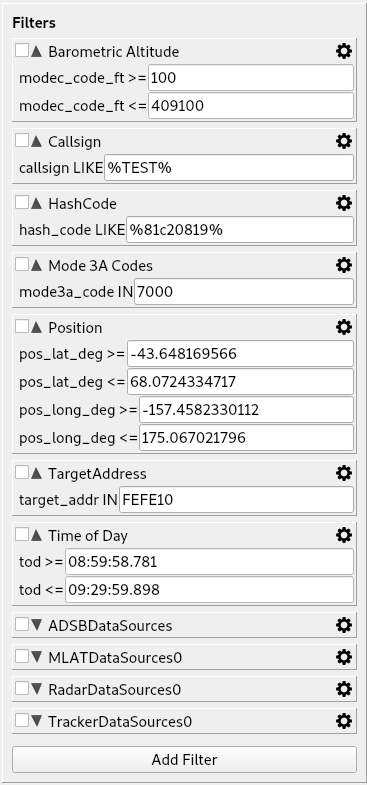
\includegraphics[width=8cm,frame]{../screenshots/filtering_details.png}
  \caption{Default Filters}
  \label{fig:filter_default}
\end{figure}

\subsection{Barometric Altitude Filter}

When active, this filter forces loading of data with a barometric altitude inside the given thresholds (in feet). Target reports without a barometric altitude will not be loaded.

\subsection{Callsign Filter}

When active, this filter forces loading of data only from callsigns matching the given expression. The percent operator denotes a 'any characters' placeholder. So e.g. '\%TEST\%' will match 'TEST123' or 'TEST123   ' (with spaces) or 'MYTEST'. Target reports without a given callsign will not be loaded.

\subsection{Mode 3/A Codes Filter}

When active, this filter forces loading of data with the given Mode A code(s), so it is possible to give multiple values (in octal notation, separated by commas). E.g. '7000' is possible, or '7000,7777'. Target reports without a given Mode A will not be loaded. \\

Please note that ADS-B target reports can also contain Mode 3/A code information.

\subsection{Position Filter}

When active, this filter forces loading of data with latitude/longitude inside the given thresholds (in degrees).

\subsection{Target Address Filter}

When active, this filter forces loading of data with the given Mode S address(es), so it is possible to give multiple values (in hexadecimal notation, irrespective of upper or lower case characters, separated by commas). E.g. 'FEFE10' is possible, or 'FEFE10,FEFE11,FEFE12'. Target reports without a given Mode S address will not be loaded.

\subsection{Time of Day Filter}

When active, this filter forces loading of data with the time-of-day inside the given thresholds (in HH:MM:SS.SSS).

\subsection{Adding a New Filter}
When clicking the 'Add filter' button, a dialog is opened.

\begin{figure}[H]
  \center
    \includegraphics[width=14cm,frame]{../screenshots/filter_add.png}
  \caption{Adding a filter}
  \label{fig:filter_add}
\end{figure}

First, one has to give the filter a new (unique) name. Then, conditions have to be defined and added. A condition consists of a DBO variable, an operator, a value, and a reset value. \\

When the triangular button is clicked, a sub-menu is opened, where one can choose a DBO variable. The selected variable restricts data of all DBOs if it is of type 'Meta', or just data from one DBO if it is not.Additionally, the mathematical operator 'ABS' can be selected. If so, not the value of the variable but the absolute value of the variable is used: 'ABS(var)>value' is equivalent to 'var>value OR var<-value'. \\

An operator can be chosen with the drop-down menu, the supplied operators are common SQL operators.

\begin{table}[H]
  \center
  \begin{tabular}{ | l | l |}
    \hline
    \textbf{Operator} & \textbf{Description} \\ \hline
    = & Equal \\ \hline
    != & Not equal \\ \hline
    > & Greater than \\ \hline
    >= & Greater than or equal \\ \hline
    < & Less than \\ \hline
    <= & Less than or equal \\ \hline
    IN & Matches a value in a comma-separated list \\ \hline
    LIKE & Pattern matching with \% and \_ \\ \hline
    IS & Value NULL: No value exists \\ \hline
    IS NOT & Value NULL: Value exists \\
    \hline
  \end{tabular}
  \caption{SQL operators}
\end{table}

In the 'Value' field one can set a value manually, or load the minimum or maximum values of the selected DBO variable from the database using the 'Load min'/'Load max' buttons . A reset value also has to be supplied, which can be the chosen value or a minimum/maximum value set from the database.  Whenever a database different from the previous one is opened, all filters are reset, since previous values may have become invalid.\\

After a condition is defined, it has to be added using the 'Add condition' button. Existing conditions are shown in the 'Current conditions' list. Please note that for now added conditions can not be removed.

\begin{figure}[H]
  \center
    \includegraphics[width=14cm,frame]{../screenshots/filter_add2.png}
  \caption{Filled out filter dialog}
  \label{fig:filter_add2}
\end{figure}

Now the described process can be repeated until a usable filter emerges, which is added using the 'Add'
button. The process of adding a new filter can be canceled by using the 'Cancel' button, which discards all
settings. When added, a new filter shows up immediately in the filter list and is saved to the configuration
for persistence.

\begin{figure}[H]
  \center
    \includegraphics[width=8cm,frame]{../screenshots/filter_add3.png}
  \caption{Filter added}
  \label{fig:filter_add3}
\end{figure}

\subsection{Managing Filters}
\label{sec:filter_management}

By clicking on the gear symbol 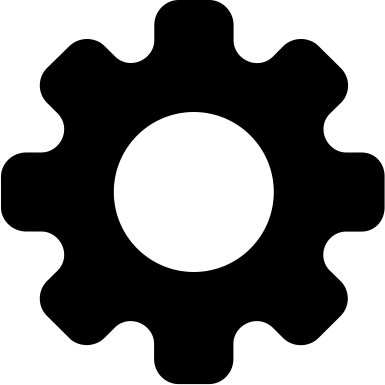
\includegraphics[scale=0.025]{../../data/icons/edit.png}, a menu allows the following operations on the filter:

\begin{itemize}  
\item Reset: Resets the filter to its default values.
\item Edit: Has been disabled and will be added at a later version.
\item Delete: Deletes a filter and permanently removes it from the configuration.
\end{itemize}
 
